\documentclass[10pt]{article}

\usepackage[portuguese]{babel}
\usepackage[utf8]{inputenc}
\usepackage[left=2cm, right=2cm, top=2cm, bottom=2cm]{geometry}
\usepackage{graphicx}
\usepackage{underscore}
\usepackage{amsmath}
\usepackage{caption}
\usepackage{textcomp}
\usepackage{float}
\usepackage{algorithm}
\usepackage[noend]{algpseudocode}
\usepackage{listings}
\lstdefinestyle{python}{
  basicstyle=\footnotesize,
  language=Python,
  numbers=none,
  stepnumber=1,
  numbersep=1pt,
  tabsize=4,
  showspaces=false,
  showstringspaces=false
}

\graphicspath{ {./images/} }

\begin{document}
\title{Relatório - Projeto 1\\
 	   MC322 - Programação Orientada a Objetos\\
 	   \textbf{Assistência e Mapeamento do COVID-19 por Municípios}
}
 	   
\author{\textbf{Grupo 13:}\\
		Airton Cardoso Lana \ \ \ \ RA: 212234\\
		Caio Vinicius Castro dos Santos \ \ \ \ RA: 214188\\
		Ian Loron de Almeida \ \ \ \ RA: 198933\\
		Murilo Gonçalves \ \ \ \ RA: 203904\\
}
\date{}

\maketitle

\section{Resumo}

\hspace{3em}\ Neste projeto objetiva-se criar um sistema que ofereça estrutura para o mapeamento e tratamento da COVID-19 a nível municipal, orientando os cidadãos que tiverem algum sintoma relacionado à doença a buscar o atendimento médico mais próximo. 

\hspace{2em}Para tal, o sistema deve fornecer uma pré-avaliação, baseada nos sintomas descritos pelo cidadão cadastrado, indicando a gravidade de seu quadro de saúde. Dessa forma, a partir de sua localização na cidade, é possível indicar qual o hospital mais próximo dessa pessoa. Ademais, a partir do diagnóstico realizado, o cidadão também será cadastrado como um paciente, dentro do sistema do hospital.

\hspace{2em}Entretanto, somente a localização não é suficiente para indicar o local mais adequado para uma pessoa buscar ajuda. Assim, também são levados em conta fatores do cidadão, como se possui convênio, e fatores do hospital, como se há disponibilidade de leitos no momento.

\hspace{2em}Assim, o mapeamento dos cidadãos será importante para indicar concentração de infectados, pessoas que estão saudáveis e pessoas que se recuperaram. Isso possibilitaria uma distribuição de recursos e insumos muito melhor, além de evitar óbitos ou casos mais graves da doença através de diagnóstico precoce, já que o cidadão não perderá tempo indo em um hospital muito longe ou em que não possa ser atendido.


\section{Funções do Sistema}
Nesta fase do projeto, o sistema é capaz de:
\begin{itemize}
\item Cadastrar cidadão;
\item Cadastrar cidade;
\item Adicionar hospital da cidade;
\item Contabilizar número de cidadãos com COVID-19;
\item Identificar suspeita de COVID-19 de um cidadão através dos sintomas que o Cidadão informar no sistema;
\item Determinar se um paciente é grupo de risco, de acordo com as informações fornecidas pelo mesmo;
\item Retornar a gravidade do quadro de saúde que o paciente tem, considerando-se o número de sintomas, a gravidade de cada sintoma e se o paciente está no quadro de risco;
\item Identificar hospital mais próximo e com leitos disponíveis a um cidadão, caso o cidadão esteja debilitado;
\item Contabilizar o período esperado de internação, dependendo do quadro de saúde do paciente;
\item Adicionar um paciente em um hospital com leitos disponíveis, de acordo com sua região, e conferindo se o paciente pode ter acesso a hospitais privados e públicos ou apenas a hospitais públicos;
\end{itemize}

Para a próxima fase do projeto, pretendemos implementar as seguintes funcionalidades:
\begin{itemize}
\item Remover hospitais da cidade;
\item Contabilizar número de casos por região da cidade;
\item Identificar quais os planos de saúde que os hospitais privados trabalham trabalham;
\item Implementar uma interface gráfica, na qual conste o mapa de uma cidade, a localização dos hospitais públicos, dos hospitais privados e dos cidadãos da cidade. Haverá marcadores coloridos com legenda para sinalizar cada localização. 
\item Controle de vacinação por região, implementando um método eficiente para vacinar as pessoas do primeiro grupo de risco. 
\end{itemize}

\section{Diagrama UML}

\begin{figure}[H]
	\centering	
    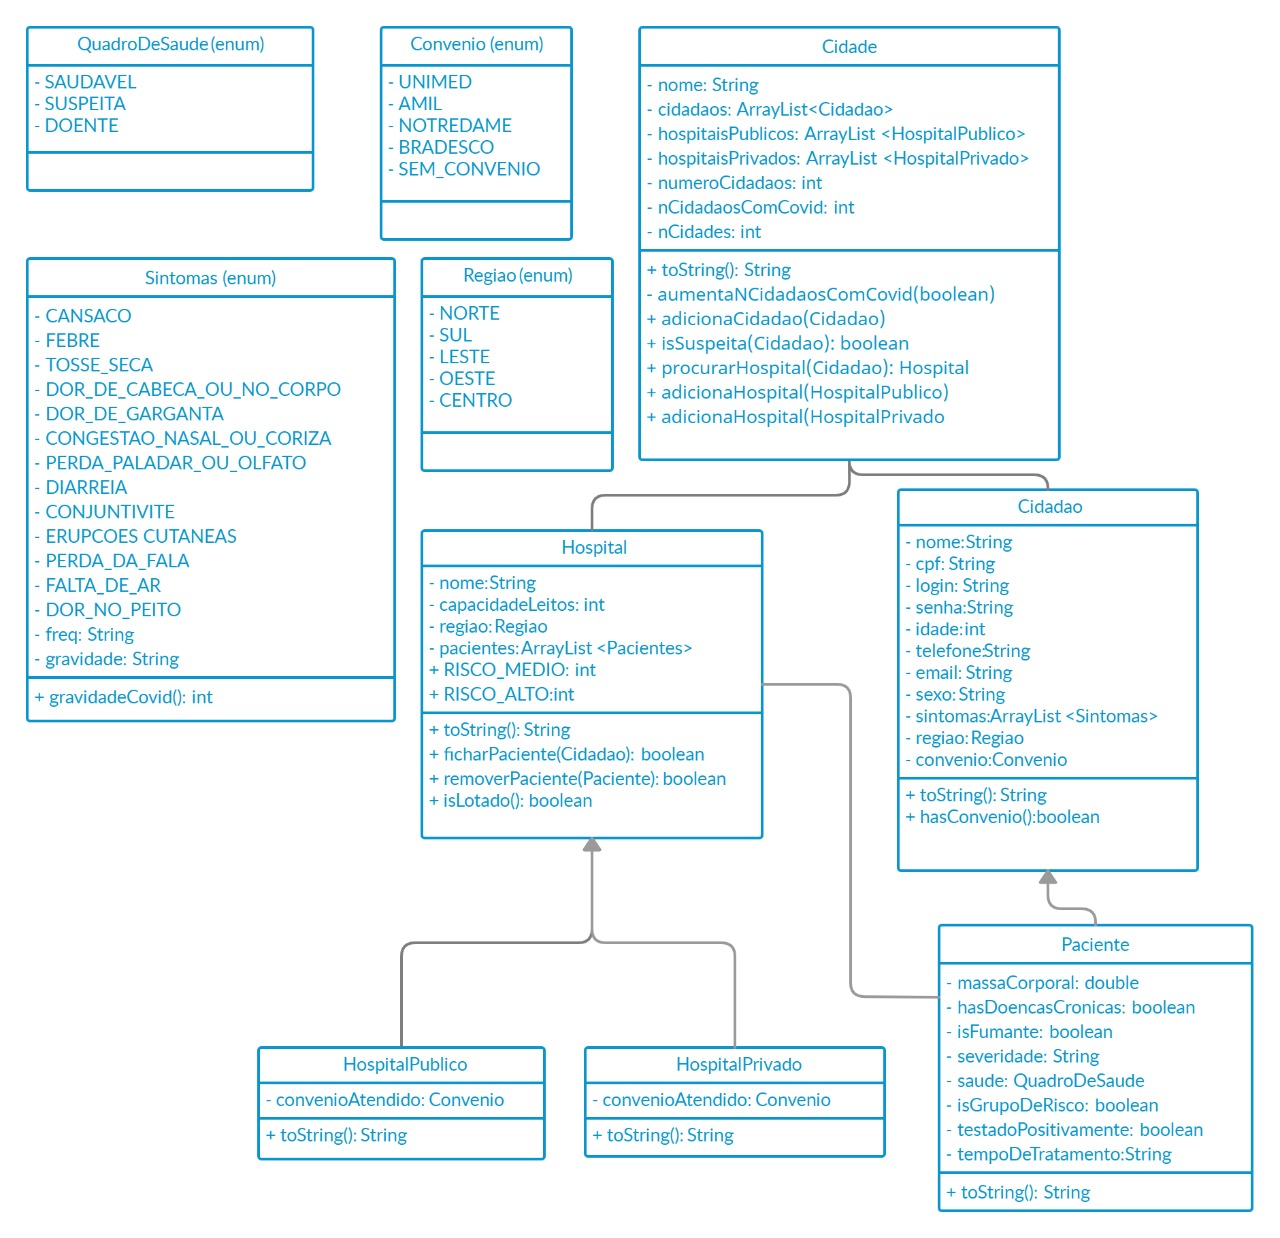
\includegraphics[width = .90\textwidth]{uml.jpg}
    \caption{UML do projeto}
\end{figure}


\end{document}